% Insert each passage at the indicated position in the team manuscript.
% The numbered sections below refer to the nine-page Team 6 report.
% For Appendix A, copy docs/pilot/paper-appendix.tex and docs/pilot/prompt.txt
% into the manuscript project, preserving their paths. See paper-appendix.tex.

% Team Contributions -- append to the existing Xichen Tang paragraph.
Xichen also prepared the common classifier inputs, ran both methods on 15
records, and calculated review agreement and classification performance.
He was responsible for the AI-assisted adjudication used to score 14 records.

% AI assistance -- append to the existing paragraph.
One provisional review used AI assistance. After inspecting the predictions,
we also used AI assistance to reconcile the supplied reviews and assign the
reference labels used in Section~4.

% Section 1.3, Labeling and data split -- replace the sentence starting
% "We will add an explicit calibration-organization exclusion check".
For the planned held-out study, we will supply the IDs of all calibration
records when we freeze the split. The freeze procedure assigns every record
from those organizations to development and rejects a supplied split that
places any of them in the test set.

% Section 2.4, Quality Assurance -- replace from "The current pipeline
% records the cutoff" through "These safeguards remain planned".
The revised freeze procedure retains supplied source URLs and rejects a
source with a known publication date after the specified cutoff. Missing
dates remain unknown. In the new cohort we will verify dates and URLs,
supply the calibration IDs, and test editing, deletion, and export/resume in
the review interface. We will also apply a common two-year evidence-age
policy to both methods. In the reported comparison, the rules screened out
old evidence before matching phrases, while the LLM interpreted the age
policy in its prompt.

% Section 4.2, Excerpt audit -- replace the two R11 sentences, preserving
% the preceding R01 correction. The verification date is after the frozen run.
The R11 excerpt described deployment in a regional academy. In a source
check on November 19, 2026, we confirmed that the full article calls the
Dra\^a-Tafilalet school-support system an experiment and attributes a
dropout-risk identification function to it. This account supports the pilot
label. The underlying parliamentary report and the system's performance
still require independent verification. The classifiers received the
original excerpts.\footnote{Hiba Chaker, \textit{Le Matin}, May 12, 2025.
\href{https://lematin.ma/nation/maroc-et-intelligence-artificielle-qui-pilote-la-machine/279065}{Article, education section}.}

% Section 4.3 -- replace the first paragraph. Retain the next paragraph
% beginning "After seeing the model outputs" with the adjudication decisions.
Of the 15 candidate records, 14 received stage labels in both supplied
reviews. One review was provisional and AI-assisted, and its notes cited
additional sources for some records. The reviews agreed on 11 of the 14
stage labels (78.6\%, unweighted Cohen's $\kappa=0.664$). This statistic
describes agreement between the two submitted reviews. R05, R06, and R08
had stage disagreements. R07 had a reason-code disagreement. For R01, the
reviews differed on eligibility and one supplied no stage label.

% Section 4.4 -- replace the two sentences from "The model was" through
% "1,500-token output cap".
We used the \texttt{gpt-4.1-mini-2025-04-14} snapshot at temperature zero
with a 1,500-token output cap.

% Appendix A -- after the existing matrices and all-15 sensitivity result,
% insert: % Add \usepackage{tikz,listings} to the manuscript preamble.
% Place the exact UTF-8 prompt at docs/pilot/prompt.txt relative to the project root.
% Include this file at the end of Appendix A with % Add \usepackage{tikz,listings} to the manuscript preamble.
% Place the exact UTF-8 prompt at docs/pilot/prompt.txt relative to the project root.
% Include this file at the end of Appendix A with % Add \usepackage{tikz,listings} to the manuscript preamble.
% Place the exact UTF-8 prompt at docs/pilot/prompt.txt relative to the project root.
% Include this file at the end of Appendix A with \input{docs/pilot/paper-appendix.tex}.
\subsection*{Classifier inputs and review sequence}
The rule baseline and the LLM each received 15 frozen packets containing
18 excerpts from 17 source URLs. In each packet, the context field was the
original short excerpt. The LLM received the same record, dates and source
metadata as the rules. Reviewers could consult fuller sources. Figure~\ref{fig:morocco-pilot-flow}
shows when the final reference labels were assigned.

\begin{figure}[htbp]
\centering
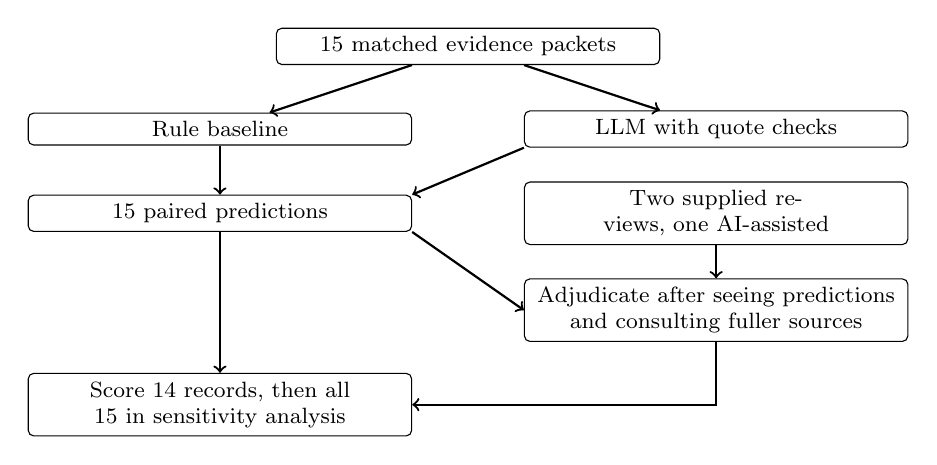
\begin{tikzpicture}[
  x=.01\linewidth,y=1cm,
  box/.style={draw,rounded corners=2pt,align=center,inner xsep=2pt,inner ysep=3pt,
              text width=.39\linewidth,font=\footnotesize},
  arr/.style={->,thick}
]
\node[box] (inputs) at (50,0) {15 matched evidence packets};
\node[box] (rules) at (24,-1.05) {Rule baseline};
\node[box] (llm) at (76,-1.05) {LLM with quote checks};
\node[box] (pred) at (24,-2.12) {15 paired predictions};
\node[box] (review) at (76,-2.12) {Two supplied reviews, one AI-assisted};
\node[box] (labels) at (76,-3.35) {Adjudicate after seeing predictions and consulting fuller sources};
\node[box] (score) at (24,-4.55) {Score 14 records, then all 15 in sensitivity analysis};
\draw[arr] (inputs) -- (rules);
\draw[arr] (inputs) -- (llm);
\draw[arr] (rules) -- (pred);
\draw[arr] (llm.south west) -- (pred.north east);
\draw[arr] (review) -- (labels);
\draw[arr] (pred.south east) -- (labels.west);
\draw[arr] (pred) -- (score);
\draw[arr] (labels.south) |- (score.east);
\end{tikzpicture}
\caption{Retrospective classification and scoring. The rules and LLM made
their predictions before the final reference labels were settled.}
\label{fig:morocco-pilot-flow}
\end{figure}

\subsection*{Exact classifier instructions}
We sent the instructions below with each request to
\texttt{gpt-4.1-mini-2025-04-14}. Each request included one evidence
packet as JSON and required a response conforming to the
\texttt{deployment\_stage} schema. The instructions assumed screened
eligibility. We later excluded R01 from the primary comparison.

\lstinputlisting[basicstyle=\ttfamily\footnotesize,breaklines=true,
  breakatwhitespace=true,columns=fullflexible,keepspaces=true,
  showstringspaces=false]{docs/pilot/prompt.txt}
.
\subsection*{Classifier inputs and review sequence}
The rule baseline and the LLM each received 15 frozen packets containing
18 excerpts from 17 source URLs. In each packet, the context field was the
original short excerpt. The LLM received the same record, dates and source
metadata as the rules. Reviewers could consult fuller sources. Figure~\ref{fig:morocco-pilot-flow}
shows when the final reference labels were assigned.

\begin{figure}[htbp]
\centering
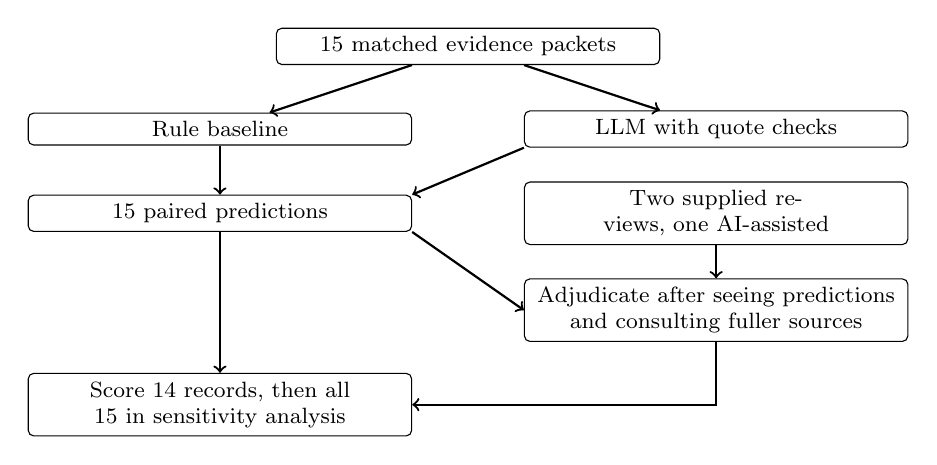
\begin{tikzpicture}[
  x=.01\linewidth,y=1cm,
  box/.style={draw,rounded corners=2pt,align=center,inner xsep=2pt,inner ysep=3pt,
              text width=.39\linewidth,font=\footnotesize},
  arr/.style={->,thick}
]
\node[box] (inputs) at (50,0) {15 matched evidence packets};
\node[box] (rules) at (24,-1.05) {Rule baseline};
\node[box] (llm) at (76,-1.05) {LLM with quote checks};
\node[box] (pred) at (24,-2.12) {15 paired predictions};
\node[box] (review) at (76,-2.12) {Two supplied reviews, one AI-assisted};
\node[box] (labels) at (76,-3.35) {Adjudicate after seeing predictions and consulting fuller sources};
\node[box] (score) at (24,-4.55) {Score 14 records, then all 15 in sensitivity analysis};
\draw[arr] (inputs) -- (rules);
\draw[arr] (inputs) -- (llm);
\draw[arr] (rules) -- (pred);
\draw[arr] (llm.south west) -- (pred.north east);
\draw[arr] (review) -- (labels);
\draw[arr] (pred.south east) -- (labels.west);
\draw[arr] (pred) -- (score);
\draw[arr] (labels.south) |- (score.east);
\end{tikzpicture}
\caption{Retrospective classification and scoring. The rules and LLM made
their predictions before the final reference labels were settled.}
\label{fig:morocco-pilot-flow}
\end{figure}

\subsection*{Exact classifier instructions}
We sent the instructions below with each request to
\texttt{gpt-4.1-mini-2025-04-14}. Each request included one evidence
packet as JSON and required a response conforming to the
\texttt{deployment\_stage} schema. The instructions assumed screened
eligibility. We later excluded R01 from the primary comparison.

\lstinputlisting[basicstyle=\ttfamily\footnotesize,breaklines=true,
  breakatwhitespace=true,columns=fullflexible,keepspaces=true,
  showstringspaces=false]{docs/pilot/prompt.txt}
.
\subsection*{Classifier inputs and review sequence}
The rule baseline and the LLM each received 15 frozen packets containing
18 excerpts from 17 source URLs. In each packet, the context field was the
original short excerpt. The LLM received the same record, dates and source
metadata as the rules. Reviewers could consult fuller sources. Figure~\ref{fig:morocco-pilot-flow}
shows when the final reference labels were assigned.

\begin{figure}[htbp]
\centering
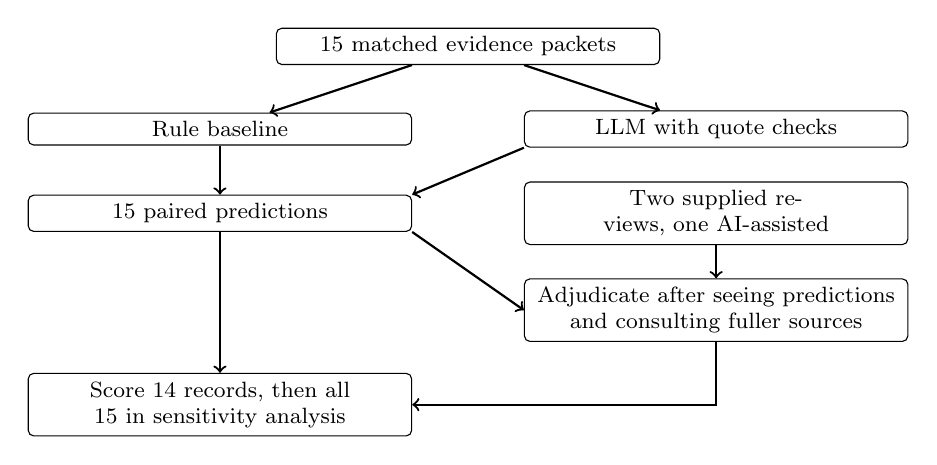
\begin{tikzpicture}[
  x=.01\linewidth,y=1cm,
  box/.style={draw,rounded corners=2pt,align=center,inner xsep=2pt,inner ysep=3pt,
              text width=.39\linewidth,font=\footnotesize},
  arr/.style={->,thick}
]
\node[box] (inputs) at (50,0) {15 matched evidence packets};
\node[box] (rules) at (24,-1.05) {Rule baseline};
\node[box] (llm) at (76,-1.05) {LLM with quote checks};
\node[box] (pred) at (24,-2.12) {15 paired predictions};
\node[box] (review) at (76,-2.12) {Two supplied reviews, one AI-assisted};
\node[box] (labels) at (76,-3.35) {Adjudicate after seeing predictions and consulting fuller sources};
\node[box] (score) at (24,-4.55) {Score 14 records, then all 15 in sensitivity analysis};
\draw[arr] (inputs) -- (rules);
\draw[arr] (inputs) -- (llm);
\draw[arr] (rules) -- (pred);
\draw[arr] (llm.south west) -- (pred.north east);
\draw[arr] (review) -- (labels);
\draw[arr] (pred.south east) -- (labels.west);
\draw[arr] (pred) -- (score);
\draw[arr] (labels.south) |- (score.east);
\end{tikzpicture}
\caption{Retrospective classification and scoring. The rules and LLM made
their predictions before the final reference labels were settled.}
\label{fig:morocco-pilot-flow}
\end{figure}

\subsection*{Exact classifier instructions}
We sent the instructions below with each request to
\texttt{gpt-4.1-mini-2025-04-14}. Each request included one evidence
packet as JSON and required a response conforming to the
\texttt{deployment\_stage} schema. The instructions assumed screened
eligibility. We later excluded R01 from the primary comparison.

\lstinputlisting[basicstyle=\ttfamily\footnotesize,breaklines=true,
  breakatwhitespace=true,columns=fullflexible,keepspaces=true,
  showstringspaces=false]{docs/pilot/prompt.txt}

